\documentclass[tikz,border=8pt]{standalone}
% Shared look for every TikZ diagram. Load with \input{../../tools/tikz-style.tex}
\usepackage[sfdefault]{roboto}
\usetikzlibrary{arrows.meta, positioning, shapes.geometric, calc, fit, backgrounds}
\definecolor{cblue}{HTML}{4C78A8}
\definecolor{corange}{HTML}{F58518}
\definecolor{cgreen}{HTML}{54A24B}
\definecolor{cred}{HTML}{E45756}
\definecolor{cpurple}{HTML}{B279A2}
\definecolor{cgrey}{HTML}{6B6B6B}
\tikzset{
  every picture/.style={font=\sffamily, line width=1.2pt},
  box/.style={draw=#1, fill=#1!12, rounded corners=4pt, align=center, inner sep=7pt, minimum height=1.1cm},
  box/.default=cgrey,
  arrow/.style={-{Stealth[length=3mm]}, draw=cgrey, line width=1.4pt},
  title/.style={font=\sffamily\bfseries\Large},
  note/.style={font=\sffamily\small, text=cgrey, align=center},
}
\AtBeginDocument{\hyphenpenalty=10000 \exhyphenpenalty=10000}

% Open loop vs closed loop for the robot's speed. Top: the force comes from the plan alone (the flat-floor
% calibration, 2 x 0.5 = 1 N); nothing measures the speed. Bottom: the wheel encoders measure the speed, the
% computer compares it with the wanted speed and adds 20 N for every m/s of error. Numbers from speedkit.py.
\begin{document}
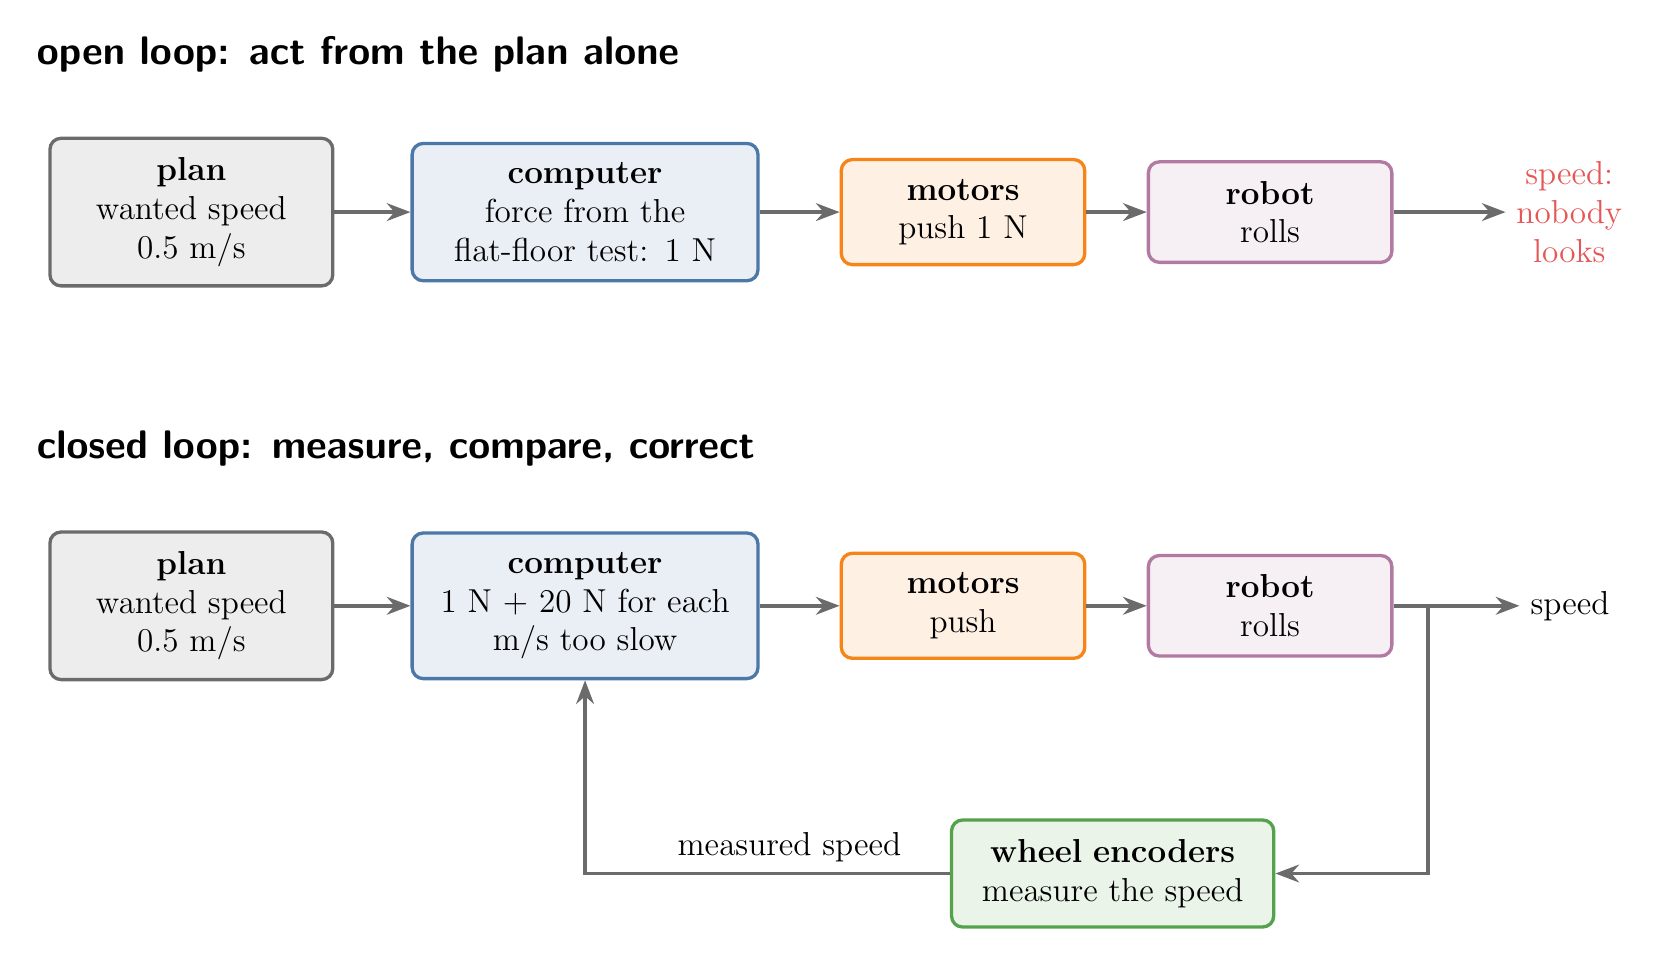
\begin{tikzpicture}[every node/.append style={font=\large}]
  \node[title, anchor=west] at (-1.2,2.0) {open loop: act from the plan alone};
  \node[box=cgrey, text width=3.1cm] (p1) at (0.9,0) {\textbf{plan}\\ wanted speed\\ 0.5 m/s};
  \node[box=cblue, text width=3.9cm] (c1) at (5.9,0) {\textbf{computer}\\ force from the\\ flat-floor test: 1 N};
  \node[box=corange, text width=2.6cm] (m1) at (10.7,0) {\textbf{motors}\\ push 1 N};
  \node[box=cpurple, text width=2.6cm] (r1) at (14.6,0) {\textbf{robot}\\ rolls};
  \node[note, font=\large, text=cred] (o1) at (18.4,0) {speed:\\ nobody\\ looks};
  \draw[arrow] (p1) -- (c1);
  \draw[arrow] (c1) -- (m1);
  \draw[arrow] (m1) -- (r1);
  \draw[arrow] (r1) -- (o1);

  \node[title, anchor=west] at (-1.2,-3.0) {closed loop: measure, compare, correct};
  \node[box=cgrey, text width=3.1cm] (p2) at (0.9,-5) {\textbf{plan}\\ wanted speed\\ 0.5 m/s};
  \node[box=cblue, text width=3.9cm] (c2) at (5.9,-5) {\textbf{computer}\\ 1 N + 20 N for each\\ m/s too slow};
  \node[box=corange, text width=2.6cm] (m2) at (10.7,-5) {\textbf{motors}\\ push};
  \node[box=cpurple, text width=2.6cm] (r2) at (14.6,-5) {\textbf{robot}\\ rolls};
  \node[box=cgreen, text width=3.6cm] (s2) at (12.6,-8.4) {\textbf{wheel encoders}\\ measure the speed};
  \draw[arrow] (p2) -- (c2);
  \draw[arrow] (c2) -- (m2);
  \draw[arrow] (m2) -- (r2);
  \draw[arrow] (r2.east) -- ++(1.6,0) node[right] {speed};
  \draw[arrow] (16.6,-5) |- (s2.east);
  \draw[arrow] (s2.west) -| node[pos=0.22, above] {measured speed} (c2.south);
\end{tikzpicture}
\end{document}
